\documentclass{article}
\usepackage{fullpage,amsthm}

\usepackage{graphicx} % support the \includegraphics command and options
\usepackage{array} % for better arrays (eg matrices) in maths
%\usepackage{paralist} % very flexible & customisable lists (eg. enumerate/itemize, etc.)
\usepackage{amsmath, amssymb, color, verbatim}
\usepackage{hyphenat,epsfig,subfigure,multirow}
\usepackage{hyperref}

\usepackage{algorithm,algorithmic}


\newtheorem{theorem}{Theorem}[section]
\newtheorem{lemma}[theorem]{Lemma}
\newtheorem{proposition}[theorem]{Proposition}
\newtheorem{corollary}[theorem]{Corollary}
\newtheorem{claim}[theorem]{Claim}
\newtheorem{fact}[theorem]{Fact}
\newtheorem{conj}[theorem]{Conjecture}
\newtheorem{definition}{Definition}[section]
%\theoremstyle{definition}
\newtheorem{remark}[theorem]{Remark}

\newenvironment{proofof}[1]{\begin{proof}[of {#1}]}{\end{proof}}

\newcommand{\mypar}[1]{\smallskip \noindent {\bf {#1}.}}
\newcommand{\myparq}[1]{\smallskip \noindent {\bf {#1}}}

\DeclareMathOperator*{\argmax}{arg\,max}
%\newenvironment{proof}[1][Proof]{\begin{trivlist}
%\item[\hskip \labelsep {\bfseries #1}]}{\end{trivlist}}
%\newenvironment{definition}[1][Definition]{\begin{trivlist}
%\item[\hskip \labelsep {\bfseries #1}]}{\end{trivlist}}
\newenvironment{example}[1][Example]{\begin{trivlist}
\item[\hskip \labelsep {\bfseries #1}]}{\end{trivlist}}
% \newenvironment{remark}[1][Remark]{\begin{trivlist}
% \item[\hskip \labelsep {\bfseries #1}]}{\end{trivlist}}

\renewcommand{\qed}{\nobreak \ifvmode \relax \else
      \ifdim\lastskip<1.5em \hskip-\lastskip
      \hskip1.5em plus0em minus0.5em \fi \nobreak
      \vrule height0.75em width0.5em depth0.25em\fi}

\newcommand{\ie}{{\it i.e.,\ }}
\newcommand{\eg}{{\it e.g.,\ }}
\newcommand{\etal}{{\it et al.\,}}
\newcommand{\through}{,\ldots,}
\newcommand{\cala}{\mathcal A}
\newcommand{\calb}{\mathcal B}
\newcommand{\calgn}{{\mathcal G}_n}
%\newcommand{\HHH}{\mathcal H}
%\newcommand{\DDD}{\mathcal D}
%\newcommand{\XXX}{\mathcal X}
\newcommand{\cals}{\mathcal S}
%\newcommand{\RRR}{\mathcal R}
\newcommand{\eps}{\epsilon}
\newcommand{\z}{\mathrm{z}}
\newcommand{\zo}{\{0,1\}}
\newcommand{\oo}{\{+1,-1\}}
\newcommand{\inv}{^{-1}}
\def\E{\mathop{\mathbb{E}}\displaylimits}
\def\poly{\mathop{\rm{poly}}\nolimits}
\def\Lap{\mathop{\rm{Lap}}\nolimits}
\newcommand{\Cauchy}{\operatorname{Cauchy}}
\newcommand{\inr}{\in_{\mbox{\tiny R}}}
\newcommand{\cP}{\mathcal P}

\title{Hierarchical Clustering for Euclidean Data}
\begin{document}
\maketitle
The goal of this project is to extend Dasgupta's hierarchical clustering paradigm to Euclidean datasets.
Recall that in the graphical case given a graph $G(V,E)$ and a tree $\mathcal T$ whose nodes correspond to vertices in the graph Dasgupta's hierarchical clustering cost is defined as follows:
$$f^-(\mathcal T) = \sum_{(i,j) \in E} w_{ij} |\{x \in T(i,j)\}|,$$
where $T(i,j)$ is the subtree of $\mathcal T$ rooted in the least common ancestor of $i$ and $j$ in $\mathcal T$.
Here $w(i,j)$ corresponds to a given similarity measure between vertices $i$ and $j$.
For the general case the best known approximation is $O(\sqrt{\log |V|})$ using the sparsest cut algorithm. Furthermore, under SSE-conjecture no algorithm can get a constant factor approximation in polynomial time~\cite{CC17}

We also consider a complementary objective which one aims to maximize:
$$f^+(\mathcal T) = \sum_{(i,j) \in E} w_{ij} (|V| - |\{x \in T(i,j)\}|),$$


Consider a set of vectors $v_1, \dots, v_n \in \mathbb R^d$. In this case the similarity measure $w$ only depends on the underlying vectors, i.e. $w_{ij} = f(v_i, v_j)$ for some function $f \colon \mathbb R \times \mathbb R \to [0,1]$.
\begin{definition}[Monotone distance-based similarity measure]
A similarity measure $w_{ij} = f(v_i, v_j)$ is \emph{distance-based} if $f(v_i, v_j) = g(\|v_i - v_j\|_2)$ for some function $g \colon \mathbb R \to [0,1]$.
A similarity measure $w_{ij}$ is \emph{monotone distance-based} if furthermore $g \colon \mathbb R \to [0,1]$ is a monotone non-increasing function.
\end{definition}

As a specific example of a monotone distance-based similarity measure it is natural to consider the Gaussian kernel similarity, i.e.: 
$$w_{ij} = (\sqrt{2 \pi} \sigma)^{-n} e^{- \frac{\|v_i - v_j\|_2^2}{2\sigma^2}},$$ 
where $\sigma$ is a normalization factor. Below we will ignore the multiplicative factor as it doesn't affect multiplicative approximations. We will also set $\sigma = 1/\sqrt{2}$ to simplify the presentation.

\textbf{Question:} Is it possible to get a better approximation and/or faster algorithm for the Hierarchical clustering problem in this setting? Or can hard instances of the general case be embedded into a into vectors with weights from the Gaussian kernel?

\section{Tight cases for Average-Linkage for $f^+$}

\subsection{High-dimensional case}
For $i \in [n^{2/3}]$ and $j \in [n^{1/3}]$ let $v_{i,j} = \Delta (e_i + (1 + \epsilon)e_{k + j})$ where $k = n^{2/3}$.
Then it is easy to see that for any fixed $i \in [n^{2/3}]$ and $j_1 \neq j_2 \in [n^{1/3}]$ it holds that:
$$\|v_{i,j_1} - v_{i, j_2}\|_2^2 = 2 (1 + \epsilon)^2 \Delta^2$$
For any fixed $j \in [n^{1/3}]$ and $i_1 \neq i_2 \in [n^{2/3}]$ it holds that:
$$\|v_{i_1, j} - v_{i_2,j}\|_2^2 = 2 \Delta^2.$$
Otherwise if $i_1 \neq i_2 \in [n^{2/3}]$ and $j_1 \neq j_2  \in [n^{1/3}]$ then:
$$\|v_{i_1, j_1} - v_{i_2, j_2}\|_2^2 = 2 \Delta^2 + 2 (1 + \epsilon)^2 \Delta^2 \ge 4 \Delta^2.$$

By setting $\Delta^2 > c \log n$ for a sufficiently large constant $c$ the contribution of pairs of vectors with $i_1 \neq i_2$ and $j_1 \neq j_2$ can be made negligible. 
The rest of the pairs correspond to an embedded hard instance from Charikar, Chatziafratis and Niazadeh (SODA'19 submission) for which average-linkage only achieves a $\frac13$-approximation compared to the optimum.

Using JL-transform we can reduce the dimension required for the above reduction to $d = O(\log n)$.

\subsection{Low-dimensional case}

For $d = 1$ the hardest instance seems to be the following.
Take four equally spaced points on a line, i.e. $0, \Delta, 2\Delta, 3 \Delta$.
Then the average-linkage clustering algorithm might first connect the two middle points and then connect the two other points in arbitrary order.
We denote the cost of this solution as $AVG$.
An alternative solution would be to create two groups $(0, \Delta)$ and $(2\Delta, 3\Delta)$ and then merge them together.
We denote the cost of this solution as $OPT$.
By making $\Delta$ sufficiently large the contribution of pairs at distance more than $\Delta$ from each other can be ignored. We thus have:
\begin{align*}
AVG \approx 3 e^{-\Delta^2} \\
OPT \approx 4 e^{- \Delta^2},
\end{align*}
which gives the ratio of $4/3$.

\textbf{Question:} Is the $4/3$ ratio achievable by average-linkage clustering for $d = 1$?


\section{Hierarchical Clustering in 1D}
We first consider the case $d = 1$.
In this case the input can be represented as points on a line, which we assume to be sorted without loss of generality, i.e. $x_1 \le \dots  \le x_n$.



\newcommand{\cblue}{\mathcal T^*_{blue}}
\newcommand{\cred}{\mathcal T^*_{red}}
\newcommand{\copt}{\mathcal T^*}
\newcommand{\cprime}{\mathcal T'^*}
\newcommand{\tblue}{T^*_{blue}}
\newcommand{\tred}{T^*_{red}}
\newcommand{\topt}{T^*}
\newcommand{\tprime}{T'^*}


\subsection{Random Cut}
Consider the following algorithm: given a range of indices $[l,r]$ pick a uniformly random index $i$ between $l$ and $r - 1$ and split the range into two: $[l, i]$ and $[i + 1, r]$, then continue recursively until the range contains a single point.
We apply this algorithm to the initial range $[1,n]$ and call it \textsc{Random Cut}.

\begin{theorem}\label{thm:random-cut-analysis}
For $d = 1$ under any monotone distance-based similarity measure $w_{ij} = g(x_i, x_j)$ the algorithm \textsc{Random Cut} gives a $\frac12$-approximation for the objective $f^+$ in expectation.
\end{theorem}
\begin{proof}
The expected value of $f^+$ for the algorithm \textsc{Random Cut} can be written as:
$$ALG = \mathbb E\left[\sum_{i = 1}^n \sum_{j = i + 1}^n w_{ij} (n - |\{x \in T(i,j)\}|)\right].$$

The rest of the analysis relies on the following two lemmas. In the first lemma we give an expression for the expected number of leaves in the subtree rooted in the least common ancestor of $i$ and $j$:
\begin{lemma}\label{lem:rand-expectation}
The random variable $T(i,j)$ corresponding to the number of leaves in the subtree rooted in the least common ancestor of $i$ and $j$ in the tree produced by the algorithm \textsc{Random Cut} has expectation:
$$\mathbb E[T(i,j)] = (j - i + 1) + \sum_{k = j + 1}^n \frac{j - i}{k - i} + \sum_{k = 1}^{i - 1} \frac{j - i}{j - k}$$
\end{lemma}
\begin{proof}
We can express $\mathbb E[T(i,j)]$ as follows:
$$\mathbb E[T_{i,j}] = \sum_{k = 1}^n \ell_k(i,j),$$
where $\ell_k$ is the probability that point $k$ belongs to the subtree rooted in the least common ancestor of $i$ and $j$.
The proof of the lemma then follows from the fact that $\ell_k$ can be expressed as:

$$
\ell_k = 
\begin{cases}
\frac{j - i}{j - k} \text{ if } k \le i - 1 \\
1 \text { if } i \le k \le j \\
\frac{j - i}{k - i} \text { if } k \ge j + 1.
\end{cases}
$$
Indeed, by construction all points between $i$ and $j$ inclusive always belong to the subtree.
Consider the case $k \le i - 1$ as the other case is symmetric. Consider the first time the segment $[k,j]$ is partitioned by the algorithm \textsc{Random Cut}.
Conditioned on $[k,j]$ being cut for the first time with probability $\frac{j - i}{j - k}$ this cut lands between $i$ and $j$ and hence $k$ belongs to the subtree and otherwise it doesn't.

\end{proof}

In the second lemma we give an upper bound on the optimum value of the objective, which we denote as $OPT$.
\begin{lemma}\label{lem:opt-bound}
For any monotone distance-based similarity measure $w$ the reward $OPT$ of the optimum solution satisfies the following inequality:
$$OPT \le \sum_{i = 1}^n \sum_{j = i + 1}^n w_{ij} (n - (j - i + 1)).$$
\end{lemma}
\begin{proof}
Consider any fixed triple of indices $(i,j,k)$ where $i < j < k$.
In the optimal tree $\mathcal T^*$  consider the least common ancestor $p$ or these three points.
Note that if we go one level below $p$ in $\mathcal T^*$ at least one of the points in the triple will get separated from the rest. This implies that only one pair in this triple can contribute to the objective and hence:
$$OPT \le \sum_{i < j < k} \max(w_{ij}, w_{ik}, w_{jk}) \le \sum_{i < j < k} \max(w_{ij}, w_{jk}),$$
where in the second inequality we use the fact that since $w$ is a monotone distance-based similarity measure it holds that $w_{ij} \ge w_{ik}$ and $w_{jk} \ge w_{ik}$.

We can now divide all $(i,j,k)$ triples into two sets:
$
\mathcal S_1 = \{(i < j < k) | w_{ij} \ge w_{jk}\} 
\mathcal S_2 = \{(i < j < k) | w_{ij} < w_{jk}\} ,
$
and hence we have:
\begin{align*}
OPT &\le \sum_{(i, j, k) \in \mathcal S_1} w_{ij} + \sum_{(i, j, k) \in \mathcal S_2} w_{jk} = \sum_{(i,j,k) \in \mathcal S_1} w_{ij} + \sum_{(k,i,j) \in \mathcal S_2} w_{ij}  \le \sum_{i < j < k} w_{ij} + \sum_{k < i < j} w_{ij} = \sum_{i < j} w_{ij} (n - (j - i + 1)).
\end{align*}
\end{proof}

We are now ready to give the proof of Theorem~\ref{thm:random-cut-analysis}.
We introduce the following notation for $i <j$: 
\begin{align*}
n_{ij} &= n - (j - i + 1) \\
e_{ij} &= n_{ij} - \sum_{k = j + 1}^n \frac{j - i}{k - i} - \sum_{k = 1}^{i - 1} \frac{j - i}{j - k}
\end{align*}
By using Lemma~\ref{lem:rand-expectation} and Lemma~\ref{lem:opt-bound} 
we have $\mathbb E[f^+(\mathcal T)] = \sum_{i = 1}^n \sum_{j = i + 1}^n w_{ij} e_{ij}$ and $OPT \le \sum_{i = 1}^n \sum_{j = i + 1}^n w_{ij} n_{ij}$.
Hence it suffices to show that:
$$\sum_{i = 1}^n \sum_{j = i + 1}^n w_{ij} e_{ij} \ge \frac12 \sum_{i = 1}^n \sum_{j = i + 1}^n w_{ij} n_{ij}.$$

%Note that the optimum solution has the following structural property.
%\begin{lemma}
%For $d = 1$ under any monotone distance-based similarity measure the optimum hierarchical clustering $\mathcal T^*$ has the property that for any pair $(i,j)$ where $i < j$ the subtree $T^*(i,j)$ rooted in the least common ancestor of $i$ and $j$ contains all the points in the range $[i,j]$.
%\end{lemma}
%\begin{proof}
%Consider the construction of $\mathcal T^*$ in a top-down fashion where we start with the root and recursively split the tree into subtrees.
%It is known (see~\cite{D16}) that the optimal clustering corresponds to a binary tree so each split creates two subtrees.
%We will represent the collection of already formed subtrees as a collection of intervals.
%
%Formally, we start with the interval $[1,n]$ and claim that after $t$ splits the already constructed subtrees correspond to a non-overlapping collection of subranges $[i_1^t, j_1^t], \dots, [i_k^t, j_k^t]$. 
%Here $k = t + 1$, $i_1^t = 1, j_k^t = n$ and for each index $\ell$ in $[1, k - 1]$ it holds that $i_{\ell + 1}^t = j_\ell^t$. 
%In order to show this claim by induction on the number of splits $t$ we need to show that for every $t$ the sequence of ranges at step $t + 1$ of the top-down splitting process is obtained by splitting one of the intervals $[i_{\ell}^t, j_\ell^t]$ for some $\ell$ into two non-overlapping subintervals.
%
%Indeed, assume for the sake of contradiction that this is not the case and some interval $[i_\ell^t, j_\ell^t]$ has been split differently into two arbitrary subsets $\mathcal R$ and $\mathcal B$ which don't correspond to non-overlapping intervals. We will refer to $\mathcal R$ as the set of \emph{red} points and $\mathcal B$ as the set of \emph{blue} points.
%W.l.o.g we can assume that $i_\ell^t \in \mathcal R$. Hence there must exist an index $r$ such that $r \in \mathcal R$ and $r - 1 \in \mathcal B$ as otherwise $\mathcal R$ and $\mathcal B$ form non-overlapping intervals. 
%
%
%
%Let $m = |\mathcal R \cup \mathcal B|$. 
%Consider moving the point $x_{r - 1}$ from $\mathcal R$ to $\mathcal B$. We denote the resulting tree as $\cprime_r$. 
%Comparing the value of the objective of the resulting tree $f^+(\cblue)$ with the objective of the optimum solution $f^+(\mathcal T^*)$ we have:
%\begin{align*}
%&f^+(\mathcal T^*) - f^+(\cblue) = \sum_{i \in [1,n] \setminus \{r - 1\}} w_{i, r - 1}(\tblue(i,r - 1) - T^*(i, r - 1)) \\
%\end{align*}
%
%Consider moving the point $x_r$ to $\mathcal B$ and the point $x_{r - 1}$ to $\mathcal R$ and then applying exactly the same partitioning on the resulting sets.
%We denote the resulting tree as $\cprime$. 
%Comparing the value of the objective of the resulting tree $f^+(\cprime)$ with the objective of the optimum solution $f^+(\mathcal T^*)$ we have:
%\begin{align*}
%&f^+(\mathcal T^*) - f^+(\cprime) = \sum_{i \in [1,n] \setminus \{r\}} w_{i,r} (T'^*(i,r) - T^*(i,r)) + \sum_{i \in [1,n] \setminus \{r - 1\}} w_{i, r - 1}(T'^*(i,r - 1) - T^*(i, r - 1)) \\
%& = \sum_{i \in \mathcal B \cup \mathcal R \setminus \{r\}}ß w_{i,r} (T'^*(i,r) - T^*(i,r)) + \sum_{i \in \mathcal B \cup \mathcal R \setminus \{r - 1\}} w_{i, r - 1}(T'^*(i,r - 1) - T^*(i, r - 1)) \\
%& = \sum_{i \in \mathcal B \cup \mathcal R \setminus \{r\}} w_{i,r} T'^*(i,r) - \sum_{i \in \mathcal B \cup \mathcal R \setminus \{r - 1\}} w_{i, r - 1} T^*(i, r - 1) 
% + \sum_{i \in \mathcal B \cup \mathcal R \setminus \{r - 1\}} w_{i, r - 1} T'^*(i,r - 1) - \sum_{i \in \mathcal B \cup \mathcal R \setminus \{r\}} w_{i,r} T^*(i, r)  \\
%&= \sum_{i \in \mathcal R \setminus \{r\}} (w_{i,r} - w_{i, r - 1}) T^*_{i,r} + \sum_{i \in \mathcal B \setminus \{r - 1\}} (w_{i,r} - w_{i, r - 1}) m 
% + \sum_{i \in \mathcal B \setminus \{r - 1\}} (w_{i,r - 1} - w_{i, r}) T^*_{i,r - 1} + \sum_{i \in \mathcal R \setminus \{r\}} (w_{i,r - 1} - w_{i, r}) m \\
%& = \sum_{i \in \mathcal R \setminus \{r\}} (w_{i,r} - w_{i, r - 1})  (T^*_{i,r} - m) + \sum_{i \in \mathcal B \setminus \{r - 1\}} (w_{i, r - 1} - w_{i, r})(T^*_{i,r - 1} - m) \\
%& \ge \sum_{i \in \mathcal R \setminus \{r\}} (w_{i,r} - w_{i, r - 1})  (T^*_{i,r} - m)
%\end{align*}
%\end{proof}



\end{proof}

\subsection{Average-Linkage}
\begin{theorem}\label{thm:average-linkage}
For $d = 1$ under any monotone distance-based similarity measure $w_{ij} = g(x_i, x_j)$ the algorithm \textsc{Average Linkage} gives a $\frac12$-approximation for the objective $f^+$.
\end{theorem}

\begin{proof}
For ease of notation from now on, for any two sets $A,B$, we denote $\sum_{i\in A,j\in B}w_{ij}$ by simply using $w_{AB}$.
The proof is based on a potential function argument. We prove that at every step, \textsc{Average Linkage} gets at least $50\%$ of the total available potential.

\begin{figure}[h!]
	\centering
	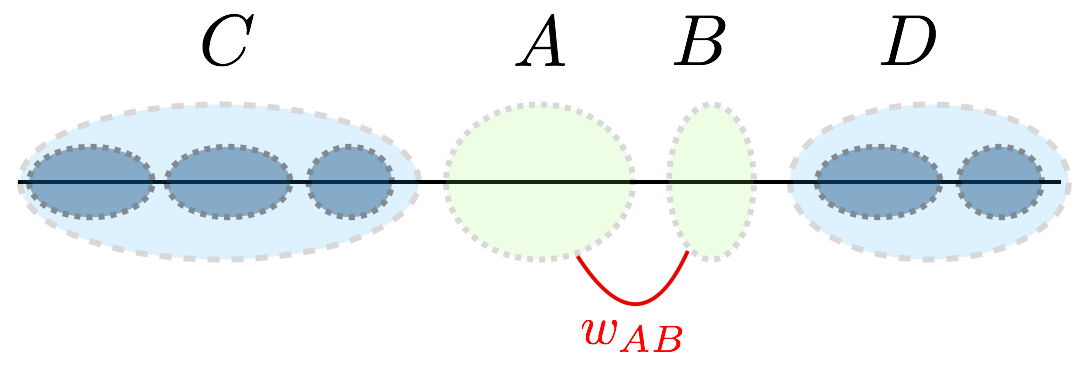
\includegraphics[width=9cm]{merging}
        	\caption{Illustration of how the merging process looks like in the 1-dimensional case.}
\end{figure}

We focus on a single step of \textsc{Average Linkage}, where neighboring clusters $A,B$ just got merged. As we see in the figure, let $C$ denote the nodes on the left of $A$ and $D$ denote the nodes on the right of $B$. Observe that $C,D$ may be empty sets. The initial total available potential is:
\[
\Phi_0 = (n-2)\sum_{e\in E}w_e
\]
 At a generic step of \textsc{Average Linkage}, by merging two clusters $A,B$, the difference in potential is:
\[
\Delta\Phi(A,B) = w_{AB}(|C|+|D|) + w_{AC}|B|+ w_{BD}|A| 
\]

By merging $A,B$, \textsc{Average Linkage} gains a contribution of:
\[
\textsc{Average Linkage}(A,B) = w_{AB}(|C|+|D|)
\]

However, after the merge, \textsc{Average Linkage} can no longer gain any contribution because of nodes in $B$ and edges between $A,C$ or because of nodes in $A$ and edges between $B,D$. More specifically, out of the total available potential at this step, $w_{AC}|B| + w_{BD}|A|$ is lost. We show that what \textsc{Average Linkage} gained at this step is no less than what \textsc{Average Linkage} lost, i.e.:
\[
w_{AB}(|C|+|D|) \ge w_{AC}|B| + w_{BD}|A|
\]

From the \textsc{Average Linkage} criterion:
\[
\dfrac{w_{AB}}{|A||B|}\ge \dfrac{w_{AC}}{|A||C|}\implies w_{AB}|C| \ge w_{AC}|B|
\]
\[
\dfrac{w_{AB}}{|A||B|}\ge \dfrac{w_{BD}}{|B||D|}\implies w_{AB}|D| \ge w_{BD}|A|
\]

By summing up we get the desired inequality which means that:
\[
\textsc{Average Linkage}(A,B)\ge \dfrac12 \Delta\Phi(A,B)
\]

At the end of the merging process, the final potential $\Phi_{n-1} = 0$, so in total:
\[
\textsc{Average Linkage}\ge \dfrac12 (n-2)\sum_{e\in E}w_e\ge \dfrac12 OPT
\]

\end{proof}

\section{Hierarchical Clustering in High Dimensions}
The input is $v_1, \dots v_n \in \mathbb R^d$. Consider an algorithm which picks a random Gaussian vector $g \sim N_d(0,1)$, projects on it and then partitions the resulting points by uniformly random cuts. Here by a uniformly random cut we mean the following process. Let $x_i = \langle v_i, g \rangle$ and assume $x_1 \le \dots \le x_n$. Pick $y \sim U([x_1, x_n])$ and split the set of points into $L = \{i \colon x_i \le y\}$ and $R = \{i \colon x_i > y\}$, then apply the same algorithm recursively on $L$ and $R$.

Fix any triangle $(v_i, v_j, v_k)$. Conditioned on cutting this triangle for the first time let $(p_{ij},p_{ik},p_{jk})$ be the vector of probabilities corresponding to the events that the corresponding edge is not cut. I.e. this is the probability that we score the contribution of this edge in the objective. Note that $p_{ij} + p_{ik} + p_{jk} = 1$.

Conisder any triangle whose vertices are $v_i, v_j, v_k$. To simplify presentation we set $i = 1, j = 2, k = 3$. We can assume that $\|v_2 - v_1\| \ge \|v_2 - v_3\| \ge \|v_1 - v_3\|$. Let $\theta_1 = \widehat{v_1 - v_3, v_2 - v_3}$, $\theta_2 = \widehat{v_2 - v_1, v_3 - v_1}$ and $\theta_3 = \widehat{v_1 - v_2, v_3 - v_2}$ so that $\theta_1 \ge \theta_2 \ge \theta_3$.

The probability that the $i$-the longest side of the triangle has the longest projection is then $\theta_i/\pi$. Conditioned on $(v_1, v_2)$ having the longest projection the probability of scoring the contribution of $(v_2, v_3)$ is given as:

$$\frac{1}{\theta_1} \int_{0}^{\theta_1} \frac{\sin \theta}{\sin (\theta + \theta_2)} \frac{\sin (\theta_1 + \theta_2)}{\sin \theta_1} d\theta $$

$$= \frac{\sin (\theta_1 + \theta_2)}{\theta_1 \sin \theta_1}\left(\theta_1 \cos \theta_2 + \ln\left(\frac{\sin \theta_2}{\sin (\theta_1 + \theta_2)}\right) \sin \theta_2 \right)$$

Now consider the probability of scoring the contribution of $(v_1,v_3)$ conditioned on $(v_1,v_2)$ having the longest projection.
We can express it as:
$$\frac{1}{\theta_1} \int_0^{\theta_1} \frac{\sin \theta}{\sin (\theta + \theta_3)} \frac{\sin(\theta_1 + \theta_3)}{\sin \theta_1} d\theta$$

It suffices to show that $\frac{\sin(\theta_1 + \theta_2)}{\sin (\theta + \theta_2)} \le \frac{\sin (\theta_1 + \theta_3)}{\sin (\theta + \theta_3)}$ for all $\theta \in [0, \theta_1]$.
Since $\theta_1 = \pi - \theta_2 - \theta_3$ this is equivalent to:
$$\frac{\sin\theta_3}{\sin (\theta + \theta_2)} \le \frac{\sin\theta_2}{\sin(\theta + \theta_3)}$$
It suffices to show that:
$$\sin\theta_3 \sin(\theta + \theta_3) \le \sin \theta_2 \sin (\theta + \theta_2)$$
Using the formula $\sin \alpha \sin \beta = \frac12(\cos(\alpha - \beta) - \cos(\alpha + \beta))$ it suffices to show that:
$$\cos(\theta + 2 \theta_3) \ge \cos(\theta + 2 \theta_2).$$
The above inequality follows for all $\theta \in [0, \pi - \theta_2 - \theta_3]$ since $\theta_3 \le \theta_2$ .

This shows that $p_{13}^{12} \ge p_{23}^{12}$. An analogous argument shows that $p_{13}^{23} \ge p_{12}^{23}$. Thus $p_{13} \ge \frac12 \frac{\theta_1 + \theta_2}{\pi} \ge \frac13$.

\bibliographystyle{alpha}
\bibliography{clustering}

\end{document}
